\documentclass[UTF8]{ctexart} %使用ctex包,中文支持
\usepackage{amsmath}  %数学公式
\usepackage{graphicx} %插图
\usepackage{fancyhdr} %个性化页眉页脚
\usepackage{geometry} %页边距
\usepackage{bm}  % 公式加粗
\usepackage{float} %为了在分栏下插入图片
\usepackage{ulem}  % 换行下划线
%\usepackage{setspace} %行间距
\usepackage{multicol} %用于实现在同一页中实现不同的分栏
\geometry{a4paper,left=2cm,right=2cm,top=2cm,bottom=2cm} % 页边距设置

\title{论文笔记}
\author{宋佳欢}
\pagestyle{plain}

\begin{document}
	
	\songti \zihao{-4}
	
	\begin{figure}[h]
	\centering
	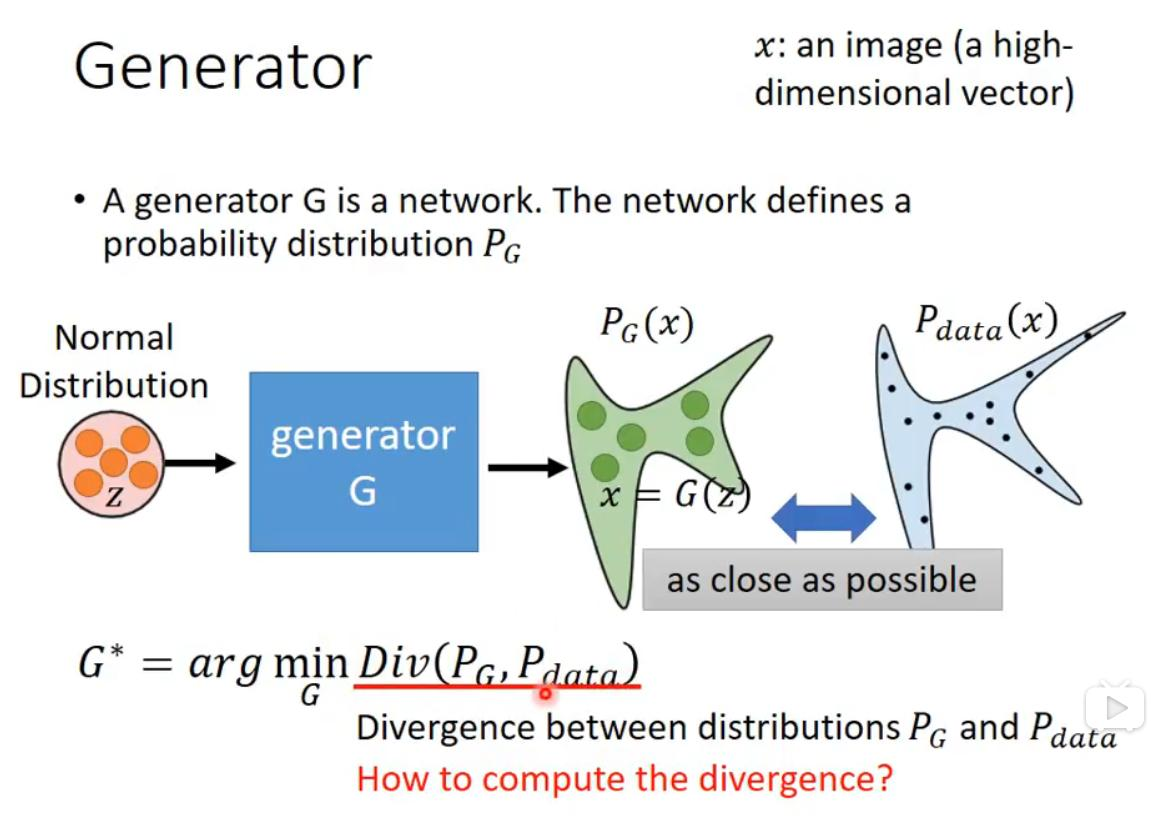
\includegraphics[scale=0.6]{screenshot001}
	\label{fig:screenshot001}
	\end{figure}
	\textbf{NIPS 2018}
	
	\zihao{3}\textbf{目的:}
	
	\zihao{-4}
	符号图推理结合卷积运算,获取全局特征;
	对符号图中的节点赋予特定的语义,比如猫狗以及它们之间的关系,而不是得到不明确的中间特征,可以人为地加入先验信息;
	节点与特征图中相关点相连,用特征图的局部特征来描述每个节点。
	\begin{figure}[H]
	\centering
	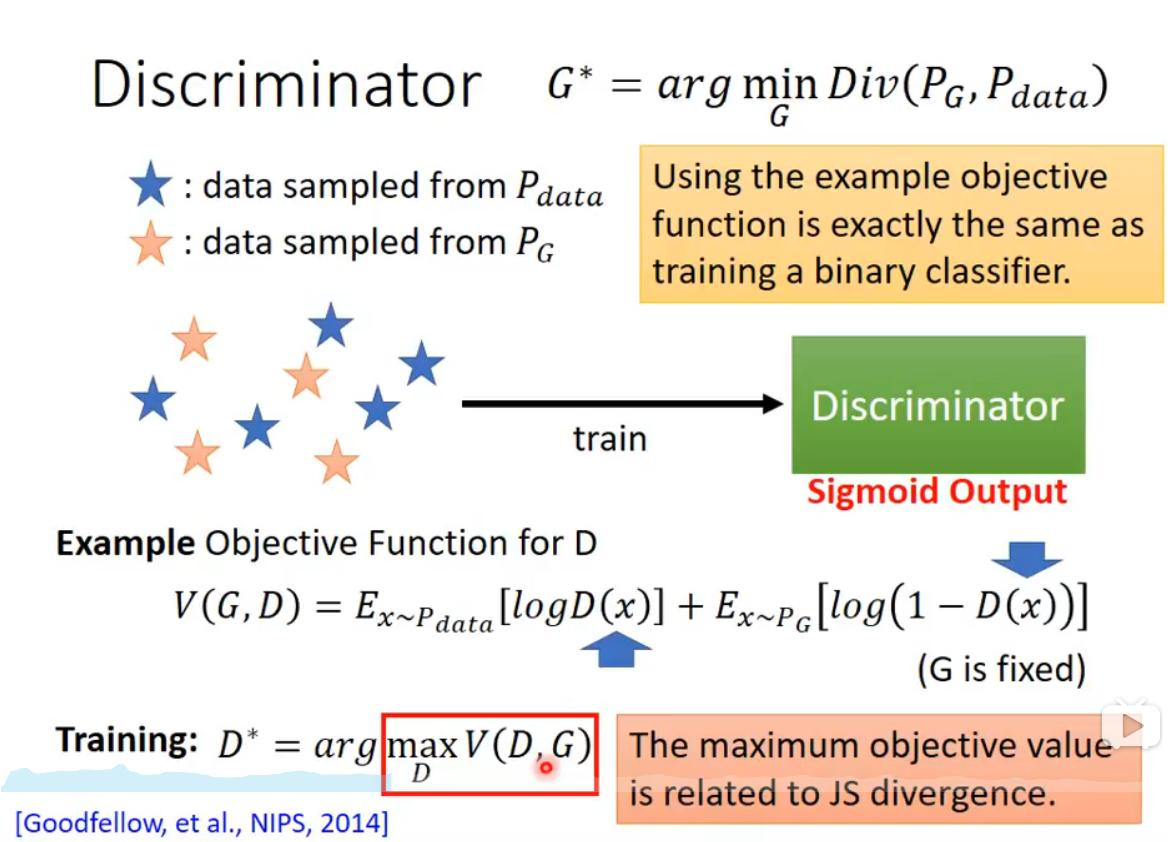
\includegraphics[scale=0.6]{screenshot002}
	\end{figure}

	\zihao{3}\textbf{方法:}
	
	\zihao{-4}
	主要包含以下3步骤:
	
	\textbf{局部特征对节点投票:}
	
	用局部特征表示每个节点。
	1*1卷积,将通道降维到节点所需空间维度;
	1*1卷积+softmax,得到特征图中每个点对M个节点的贡献系数;
	然后每个节点就可表示成特征图中的点的线性组合;
	
	这一步和A2Net中的第一步相同,相当于低秩重建中的降秩。

	\textbf{图推理:}
	
	首先将词嵌入向量与上个模块的得到的节点特征表示向量拼接起来,然后再每一维度线性组合,降维到节点原来的维度;
	引入一个人为确定的图,代表各个节点之间的关系,对这个矩阵对称归一化,然后在对这些节点重新组合。
	
	\textbf{使用节点语义增强局部特征:}
	
	用1*1卷积将节点维度在恢复到原特征图通道大小;
	为了对每个特征点选择合适的节点对齐增强,这里用了相似性度量,具体看图2,最后得到M个节点对每个特征点的权重(贡献程度)
	然后用这些权重和节点,重组特征图;
	然后残差连接。
	
	\begin{figure}[H]
	\centering
	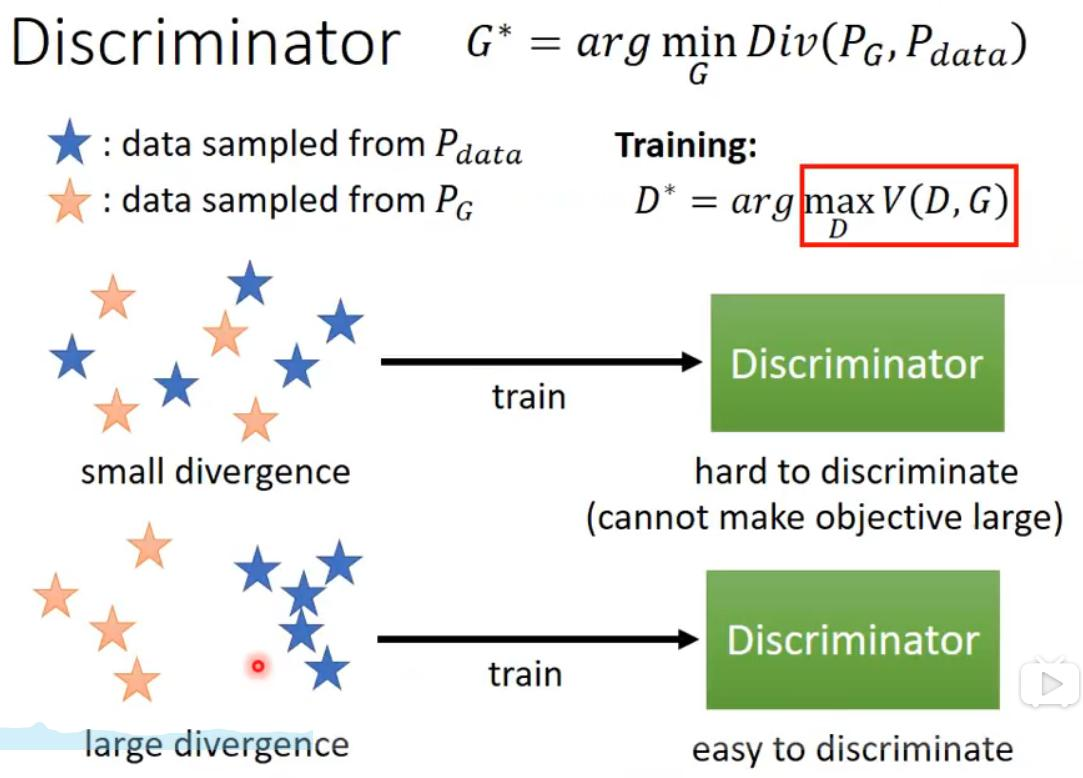
\includegraphics[scale=0.6]{screenshot003}
	\end{figure}
	
	
	\zihao{3}\textbf{总结:}
	
	\zihao{-4}
		我感觉文章的想法非常好也是很直觉的,加入图的推断,将具体的某些物体或者特性联系起来,作为一个先验信息,用卷积得到的视觉特征与图中设定物体匹配,这就有点像人在日常生活中识别物体一样。但是文中并没有对图中的节点做具体的可视化等分析,可能性能的提升只是由于对特征的低秩重建的结构。
		
		
\end{document}